\documentclass[11pt,t,usepdftitle=false,aspectratio=169,usenames,dvipsnames]{beamer}
\usetheme[nototalframenumber,foot,logo]{uibk}
\headerimage{3}

\usepackage[T1]{fontenc}
\usepackage{xcolor}
\usepackage{minted}
\usepackage{tikz}
\usetikzlibrary{calc}

\definecolor{uibkBlue}{HTML}{00325c}
\definecolor{uibkOrange}{HTML}{ff9027}

\title{Reimplementing CoAP for C\# with the Task-based Asynchronous Pattern}
\subtitle{Is it worth to await?}
\author{Philip Wille}

\begin{document}
    \maketitle{}

    \begin{frame}
        \frametitle{Introduction}
        \begin{itemize}
            \item<1-> Synchronous and asynchronous execution
            \begin{itemize}
                \item<2-> Synchronous:
                \begin{itemize}
                    \item<3-> \textcolor{uibkBlue}{\textbf{Waiting for completion}} of method before continuing with program flow.
                    \item<5-> \textcolor{uibkBlue}{\textbf{Busy waiting}} $\rightarrow$ Thread is marked as \textcolor{uibkBlue}{\textbf{blocked}}.
                \end{itemize}
                \item<2-> Asynchronous:
                \begin{itemize}
                    \item<4-> Can \textcolor{uibkBlue}{\textbf{perform other tasks}} while the execution is running.
                    \item<6-> The main thread will be \textcolor{uibkBlue}{\textbf{notified}}.
                    \item<7-> \textcolor{uibkBlue}{\textbf{No busy waiting}} $\rightarrow$ Thread is \textcolor{uibkBlue}{\textbf{free}} for other tasks.
                \end{itemize}
            \end{itemize}
            \item<8-> \textcolor{uibkBlue}{\textbf{T}}ask-based \textcolor{uibkBlue}{\textbf{A}}synchronous \textcolor{uibkBlue}{\textbf{P}}attern (TAP)
            \begin{itemize}
                \item<9-> Developed by Microsoft.
                \item<10-> Small changes to synchronous code for enabling asynchronous execution.
                \item<11-> Built-in in C\#.
            \end{itemize}
            \item<12-> \textcolor{uibkBlue}{\textbf{Co}}nstrained \textcolor{uibkBlue}{\textbf{A}}pplication \textcolor{uibkBlue}{\textbf{P}}rotocol (CoAP)
            \begin{itemize}
                \item<13-> Designed for \textcolor{uibkBlue}{\textbf{M}}achine-\textcolor{uibkBlue}{\textbf{t}}o-\textcolor{uibkBlue}{\textbf{M}}achine (M2M) devices.
                \item<14-> Request/response interaction model.
            \end{itemize}
        \end{itemize}
    \end{frame}

    \begin{frame}
        \frametitle{Synchronous server}
        \begin{figure}[ht]
            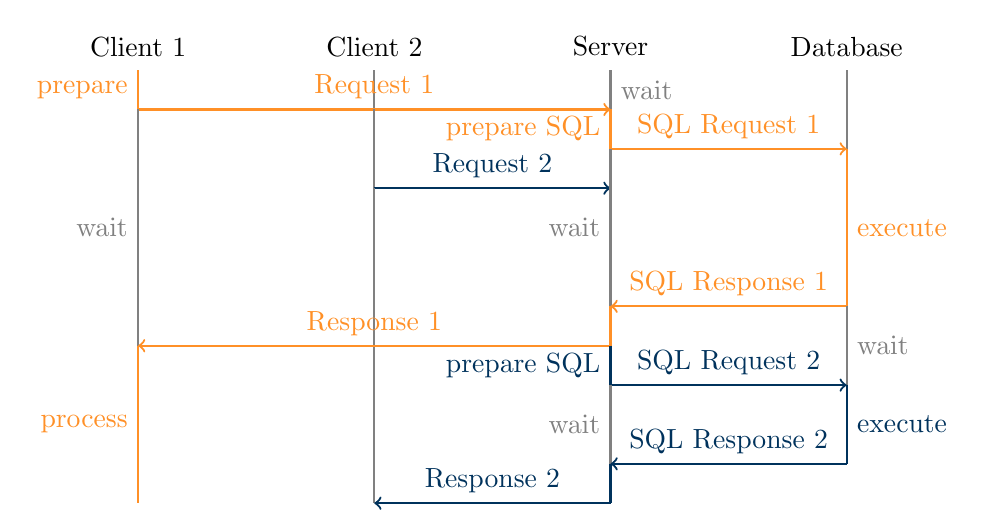
\begin{tikzpicture}
                \node at (0,.3) {Database};
                \node at (-3,.3) {Server};
                \node at (-6,.3) {Client 2};
                \node at (-9,.3) {Client 1};
                
                \draw[thick, uibkOrange] (-9,0) -- node[left] {prepare}(-9,-0.5);
                \draw[thick, gray] (-6,0) -- (-6,-0.5);
                \draw[thick, gray] (-3,0) -- node[right, midway] {wait} (-3,-0.5);
                \draw[thick, gray] (-0,0) -- (0,-1);
                \onslide<1->
                \draw[->, thick, uibkOrange] (-9,-0.5) -- node[midway,above] {Request 1} (-3,-0.5);
                \onslide<2->
                \draw[thick, uibkOrange] (-3,-0.5) -- node[left] {prepare SQL}(-3,-1);
                \draw[thick, gray] (-6,-0.5) -- (-6,-1.5);
                \draw[thick, gray] (-9,-0.5) -- node[left] {wait} (-9,-3.5);
                \onslide<3->
                \draw[->, thick, uibkOrange] (-3,-1) -- node[midway,above] {SQL Request 1} (-0,-1);
                \onslide<4->
                \draw[thick, uibkOrange] (-0,-1) -- node [right] {execute} (0,-3);
                \draw[->, thick, uibkBlue] (-6,-1.5) -- node[midway,above] {Request 2} (-3,-1.5);
                \draw[thick, gray] (-3,-1) -- node [left] {wait} (-3,-3);
                \draw[thick, gray] (-6,-1.5) -- (-6,-5.5);
                \onslide<5->
                \draw[<-, thick, uibkOrange] (-3,-3) -- node [midway, above] {SQL Response 1} (0,-3);
                \onslide<6->
                \draw[thick, uibkOrange] (-3,-3) -- (-3,-3.5);
                \onslide<7->
                \draw[<-, thick, uibkOrange] (-9,-3.5) -- node [midway, above] {Response 1} (-3,-3.5);
                \onslide<8->
                \draw[thick, uibkOrange] (-9,-3.5) -- node [midway, left] {process} (-9,-5.5);
                \draw[thick, uibkBlue] (-3,-3.5) -- node [midway, left] {prepare SQL} (-3,-4);
                \draw[thick, gray] (-0,-3) -- node [midway, right] {wait} (-0,-4);
                \onslide<9->
                \draw[->, thick, uibkBlue] (-3,-4) -- node [midway, above] {SQL Request 2} (-0,-4);
                \onslide<10->
                \draw[thick, uibkBlue] (-0,-4) -- node [midway, right] {execute} (-0,-5);
                \onslide<11->
                \draw[thick, gray] (-3,-4) -- node [midway, left] {wait} (-3,-5);
                \draw[<-, thick, uibkBlue] (-3,-5) -- node [midway, above] {SQL Response 2} (-0,-5);
                \onslide<12->
                \draw[thick, uibkBlue] (-3,-5) -- (-3,-5.5);
                \onslide<13->
                \draw[<-, thick, uibkBlue] (-6,-5.5) -- node [midway, above] {Response 2} (-3,-5.5);
            \end{tikzpicture}
        \end{figure}
    \end{frame}

    \begin{frame}
        \frametitle{Asynchronous server}
        \begin{figure}[ht]
            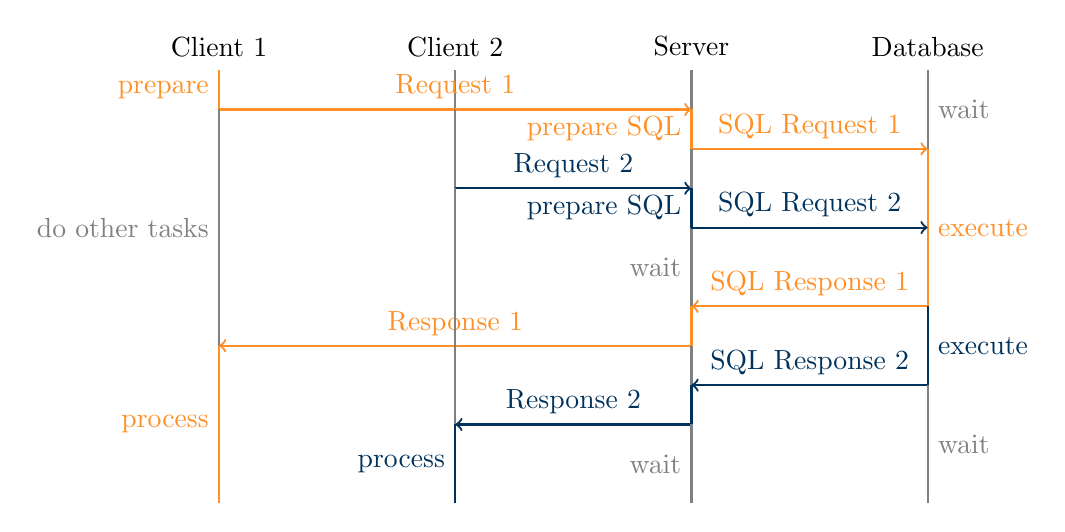
\begin{tikzpicture}
                \node at (0,.3) {Database};
                \node at (-3,.3) {Server};
                \node at (-6,.3) {Client 2};
                \node at (-9,.3) {Client 1};
                
                \draw[thick, uibkOrange] (-9,0) -- node[left] {prepare}(-9,-0.5);
                \draw[thick, gray] (-6,0) -- (-6,-0.5);
                \draw[thick, gray] (-3,0) -- (-3,-0.5);
                \draw[thick, gray] (-0,0) -- node[right, midway] {wait} (0,-1);
                \draw[->, thick, uibkOrange] (-9,-0.5) -- node[midway,above] {Request 1} (-3,-0.5);
                \draw[thick, uibkOrange] (-3,-0.5) -- node[left] {prepare SQL}(-3,-1);
                \draw[thick, gray] (-6,-0.5) -- (-6,-1.5);
                \draw[thick, gray] (-9,-0.5) -- node[left] {do other tasks} (-9,-3.5);
                \draw[->, thick, uibkOrange] (-3,-1) -- node[midway,above] {SQL Request 1} (-0,-1);
                \draw[thick, uibkOrange] (-0,-1) -- node [right] {execute} (0,-3);
                \draw[->, thick, uibkBlue] (-6,-1.5) -- node[midway,above] {Request 2} (-3,-1.5);
                \draw[thick, gray] (-3,-1) -- (-3,-1.5);
                \draw[thick, uibkBlue] (-3,-1.5) -- node[midway, left] {prepare SQL} (-3,-2);
                \draw[thick, gray] (-3,-2) -- node[midway, left] {wait} (-3,-3);
                \draw[<-, thick, uibkOrange] (-3,-3) -- node [midway, above] {SQL Response 1} (0,-3);
                \draw[thick, uibkOrange] (-3,-3) -- (-3,-3.5);
                \draw[<-, thick, uibkOrange] (-9,-3.5) -- node [midway, above] {Response 1} (-3,-3.5);
                \draw[thick, uibkOrange] (-9,-3.5) -- node [midway, left] {process} (-9,-5.5);
                \draw[thick, uibkBlue] (-0,-3) -- node [midway, right] {execute} (-0,-4);
                \draw[->, thick, uibkBlue] (-3,-2) -- node [midway, above] {SQL Request 2} (-0,-2);
                \draw[thick, gray] (-3,-3.5) -- (-3,-4);
                \draw[<-, thick, uibkBlue] (-3,-4) -- node [midway, above] {SQL Response 2} (-0,-4);
                \draw[thick, uibkBlue] (-3,-4) -- (-3,-4.5);
                \draw[thick, gray] (0,-4) -- node [midway, right] {wait} (0,-5.5);
                \draw[thick, gray] (-6,-1.5) -- (-6,-4.5);
                \draw[<-, thick, uibkBlue] (-6,-4.5) -- node [midway, above] {Response 2} (-3,-4.5);
                \draw[thick, uibkBlue] (-6,-4.5) -- node [midway, left] {process} (-6,-5.5);
                \draw[thick, gray] (-3,-4.5) -- node [midway, left] {wait} (-3,-5.5);
            \end{tikzpicture}
        \end{figure}
    \end{frame}

    \begin{frame}
        \frametitle{Synchronous execution in C\#}
        
        \begin{listing}[H]
            \inputminted[framesep=2mm, baselinestretch=1.2, fontsize=\scriptsize, linenos]{csharp}{codes/example_synchronous.cs}
            \caption{Synchronous usage in C\#}
            \label{listing:asynchronous-usage-in-csharp}
        \end{listing}
    \end{frame}

    \begin{frame}
        \frametitle{Execute synchronous code asynchronously in C\#}

        \begin{listing}[H]
            \inputminted[framesep=2mm, baselinestretch=1.2, fontsize=\scriptsize, linenos]{csharp}{codes/example_synchronous_code_asynchronously.cs}
            \caption{Synchronous code executed asynchronously in C\#}
            \label{listing:synchronous-code-executed-asynchronously-in-csharp}
        \end{listing}
    \end{frame}

    \begin{frame}
        \frametitle{Event-based execution in C\#}
        
        \begin{listing}[H]
            \inputminted[framesep=2mm, baselinestretch=1.2, fontsize=\scriptsize, linenos, lastline=15]{csharp}{codes/example_eventbased.cs}
            \caption{DownloadResult to get string}
            \label{listing:download-result-to-get-string}
        \end{listing}
    \end{frame}

    \begin{frame}
        \frametitle{Event-based execution in C\#}
        
        \begin{listing}[H]
            \inputminted[framesep=2mm, baselinestretch=1.2, fontsize=\scriptsize, linenos, firstline=17]{csharp}{codes/example_eventbased.cs}
            \caption{Usage of events in C\#}
            \label{listing:usage-of-events-in-csharp}
        \end{listing}
    \end{frame}

    \begin{frame}
        \frametitle{Asynchronous execution in C\#}

        \begin{listing}[H]
            \inputminted[framesep=2mm, baselinestretch=1.2, fontsize=\scriptsize, linenos]{csharp}{codes/example_asynchronous.cs}
            \caption{Asynchronous usage in C\#}
            \label{listing:asynchronous-usage-in-csharp}
        \end{listing}
    \end{frame}

    \begin{frame}
        \frametitle{Short introduction into CoAP}

        \begin{itemize}
            \item URI scheme based
            \begin{itemize}
                \item "coap:" "//" host [ ":" port ] path-abempty [ "?" query ]
                \item "coaps:" "//" host [ ":" port ] path-abempty [ "?" query ]
            \end{itemize}
            \item REST-like
            \begin{itemize}
                \item GET, PUT, POST, DELETE, PATCH, ...
            \end{itemize}
            \item Specialized for using with constrained nodes and constrained networks.
            \item Works with HTTP.
            \item Fulfills requirements of environments like energy, building automation, and other machine-to-machine (M2M) applications.
            \item Several implementations for many programming languages like C\# (CoAP.NET), Java (Californium), Python (CoAPthon), C (FreeCoAP) ...
        \end{itemize}
    \end{frame}

    \begin{frame}
        \frametitle{Example request in CoAP}

        \begin{figure}[ht]
            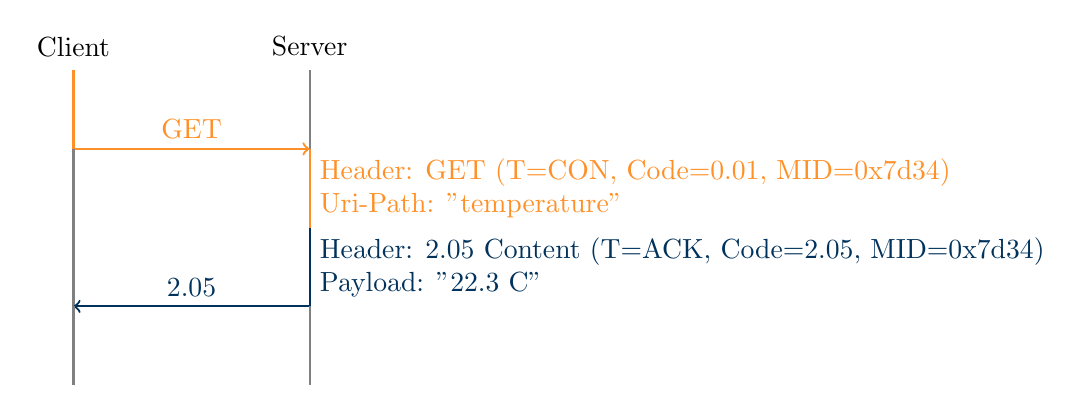
\begin{tikzpicture}
                \node at (-3,.3) {Client};
                \node at (0,.3) {Server};

                \draw[thick, uibkOrange] (-3,0) -- (-3,-1);
                \draw[thick, gray] (0,0) -- (0,-1);
                \onslide<1->
                \draw[->, thick, uibkOrange] (-3,-1) -- node[midway,above] {GET} (0,-1);
                \onslide<2->
                \draw[thick, gray] (-3,-1) -- (-3,-2);
                \draw[thick, uibkOrange] (0,-1) -- node[right, align=left] {Header: GET (T=CON, Code=0.01, MID=0x7d34)\\Uri-Path: "temperature"} (0,-2);
                \onslide<3->
                \draw[thick, gray] (-3,-1) -- (-3,-3);
                \draw[thick, uibkBlue] (0,-2) -- node[right, align=left] {Header: 2.05 Content (T=ACK, Code=2.05, MID=0x7d34)\\Payload: "22.3 C"} (0,-3);
                \draw[<-, thick, uibkBlue] (-3,-3) -- node[midway,above] {2.05} (0,-3);
                \onslide<4->
                \draw[thick, gray] (-3, -3) -- (-3, -4);
                \draw[thick, gray] (0, -3) -- (0, -4);
            \end{tikzpicture}
            \caption{GET request}
            \label{example-get-request}
        \end{figure}
    \end{frame}

    \begin{frame}
        \frametitle{CoAP.NET}

        \begin{itemize}
            \item Implementation of CoAP for C\#.
            \item Development inactive.
            \item Partially asynchronous.         
        \end{itemize}
    \end{frame}

    \begin{frame}
        \frametitle{Goal thesis}

        \begin{itemize}
            \item Goals
            \begin{itemize}
                \item Rewrite CoAP.NET to fully asynchronous version.
                \item Fixing memory leaks.
                \item Enhancing diagnostic capabilities.
                \item Upgrading to .NET Standard 2.0.
                \item Several improvements.
            \end{itemize}
            \item Supervisors
            \begin{itemize}
                \item assoc. Prof. Dr. Michael Felderer (University Innsbruck).
                \item Andreas Dânek (World-Direct eBusiness solutions GmbH)
            \end{itemize}
        \end{itemize}
    \end{frame}
\end{document}